\documentclass[14pt]{article}
\usepackage{../../report-tex/styles}

\begin{document}

\titlewithlabnum{2}

\tableofcontents
\newpage

\section{Мета:}
отримати вміння та навички використовувати інкапсуляцію,
абстракцію типів, успадкування та поліморфізм на основі класів С++,
запрограмувавши простий графічний редактор в об’єктно-орієнтованому
стилі.
\section{Завдання:}
\begin{enumerate}
    \item Створити у середовищі MS Visual Studio C++ проект типу Windows Desktop Application з ім’ям Lab2.
    \item Скомпілювати проект і отримати виконуваний файл програми.
    \item Перевірити роботу програми. Налагодити програму.
    \item Проаналізувати та прокоментувати результати та вихідний текст програми.
    \item Оформити звіт.
\end{enumerate}

\subsection{Варіанти завдань та основні вимоги}
1. Для усіх варіантів завдань необхідно дотримуватися вимог та
положень, викладених вище у порядку виконання роботи та методичних
рекомендаціях. \\
2. У звіті повинна бути схема успадкування класів – діаграма класів \\
3. Для вибору типу об’єкта в графічному редакторі Lab2 повинно бути
меню "Об’єкти" з чотирма підпунктами. Меню "Об’єкти" повинно бути
праворуч меню "Файл" та ліворуч меню "Довідка". Підпункти меню
"Об’єкти" містять назви українською мовою геометричних форм – так, як
наведено вище у порядку виконання роботи та методичних рекомендаціях.
Геометричні форми згідно варіанту завдання. \\
4. Для вибору варіанту використовується Ж – номер студента в
журналі. \\
5. Масив вказівників для динамічних об’єктів типу Shape
- динамічний масив Shape **pcshape;
- статичний масив Shape *pcshape[N];
причому, кількість елементів масиву вказівників як для статичного, так і
динамічного має бути N = Ж+100.
Динамічний масив обирають студенти, у яких варіант (Ж mod 3 = 0).
Решта студентів – статичний масив. Позначка mod означає залишок від
ділення. \\
6. "Гумовий" слід при вводі об’єктів
- суцільна лінія чорного кольору для варіантів (Ж mod 4 = 0) \\
- суцільна лінія червоного кольору для варіантів (Ж mod 4 = 1) \\
- суцільна лінія синього кольору для варіантів (Ж mod 4 = 2) \\
- пунктирна лінія чорного кольору для варіантів (Ж mod 4 =3) \\
7. Чотири геометричні форми (крапка, лінія, прямокутник, еліпс)
можуть мати наступні різновиди вводу та відображення. \\
7.1. Прямокутник
Увід прямокутника:
- по двом протилежним кутам для варіантів (Ж mod 2 = 0)
- від центру до одного з кутів для варіантів (Ж mod 2 = 1)
Відображення прямокутника:
- чорний контур з білим заповненням для (Ж mod 5 = 0)
- чорний контур з кольоровим заповненням для (Ж mod 5 = 1 або 2)
- чорний контур прямокутника без заповнення для (Ж mod 5 = 3 або 4)
Кольори заповнення прямокутника:
- жовтий для (Ж mod 6 = 0)
- світло-зелений для (Ж mod 6 = 1)
- блакитний для (Ж mod 6 = 2)
- рожевий для (Ж mod 6 = 3)
- померанчевий для (Ж mod 6 = 4)
- сірий для (Ж mod 6 = 5) \\
7.2. Еліпс
Увід еліпсу:
- по двом протилежним кутам охоплюючого прямокутника для
варіантів (Ж mod 2 = 1)
- від центру до одного з кутів охоплюючого прямокутника для варіантів
(Ж mod 2 = 0)
Відображення еліпсу:
- чорний контур з білим заповненням для (Ж mod 5 = 1)
- чорний контур з кольоровим заповненням для (Ж mod 5 = 3 або 4)
- чорний контур еліпсу без заповнення для (Ж mod 5 = 0 або 2)
Кольори заповнення еліпсу:
- жовтий для (Ж mod 6 = 1)
- світло-зелений для (Ж mod 6 = 2)
- блакитний для (Ж mod 6 = 3)
- рожевий для (Ж mod 6 = 4)
- померанчевий для (Ж mod 6 = 5)
- сірий для (Ж mod 6 = 0) \\
8. Позначка поточного типу об’єкту, що вводиться
- в меню (метод OnInitMenuPopup) для варіантів (Ж mod 2 = 0)
- в заголовку вікна для (Ж mod 2 = 1) \\
9. Приклад вибору варіанту. Для 9-го студента у списку (Ж = 9) буде:
- динамічний масив для Shape (9 mod 3 = 0) обсягом 109 об’єктів
- "гумовий" слід (9 mod 4 = 1) – суцільна лінія червоного кольору
- прямокутник:
- ввід від центру до одного з кутів (9 mod 2 = 1)
- чорний контур прямокутника без заповнення (9 mod 5 = 4)
- еліпс:
- по двом протилежним кутам охопл. прямокутника(9 mod 2 = 1)
- чорний контур з кольоровим заповненням (9 mod 5 = 4)
- колір заповнення: блакитний (9 mod 6 = 3)
- позначка поточного типу об’єкту: в заголовку вікна (9 mod 2 = 1)
Примітка. Визначення кольорів та інші параметри варіантів можуть
бути змінені викладачем шляхом оголошення студентам відповідного
повідомлення завчасно перед постановкою завдань.


\section{Текст програми:}
\subsection{Module: com.github.erotourtes.drawing.editor}
\lstinputlistingukr{DmProcessor.kt}{../src/main/kotlin/com/github/erotourtes/drawing/editor/DmProcessor.kt}
\lstinputlistingukr{Editor.kt}{../src/main/kotlin/com/github/erotourtes/drawing/editor/Editor.kt}
\lstinputlistingukr{Editors.kt}{../src/main/kotlin/com/github/erotourtes/drawing/editor/Editors.kt}
\lstinputlistingukr{ShapesList.kt}{../src/main/kotlin/com/github/erotourtes/drawing/editor/ShapesList.kt}

\subsection{Module: 1.0}
\lstinputlistingukr{MANIFEST.MF}{../src/main/resources/META-INF/MANIFEST.MF}

\subsection{Module: com.github.erotourtes.view}
\lstinputlistingukr{MainController.kt}{../src/main/kotlin/com/github/erotourtes/view/MainController.kt}
\lstinputlistingukr{MainView.kt}{../src/main/kotlin/com/github/erotourtes/view/MainView.kt}
\lstinputlistingukr{MenuBar.kt}{../src/main/kotlin/com/github/erotourtes/view/MenuBar.kt}
\lstinputlistingukr{ToolBar.kt}{../src/main/kotlin/com/github/erotourtes/view/ToolBar.kt}

\subsection{Module: com.github.erotourtes.app}
\lstinputlistingukr{MyApp.kt}{../src/main/kotlin/com/github/erotourtes/app/MyApp.kt}

\subsection{Module: com.github.erotourtes.drawing}
\lstinputlistingukr{CanvasPane.kt}{../src/main/kotlin/com/github/erotourtes/drawing/CanvasPane.kt}
\lstinputlistingukr{EditorHandler.kt}{../src/main/kotlin/com/github/erotourtes/drawing/EditorHandler.kt}

\subsection{Module: com.github.erotourtes.drawing.shape}
\lstinputlistingukr{Shape.kt}{../src/main/kotlin/com/github/erotourtes/drawing/shape/Shape.kt}
\lstinputlistingukr{Shapes.kt}{../src/main/kotlin/com/github/erotourtes/drawing/shape/Shapes.kt}

\subsection{Module: com.github.erotourtes.styles}
\lstinputlistingukr{ToolbarStyles.kt}{../src/main/kotlin/com/github/erotourtes/styles/ToolbarStyles.kt}

\subsection{Module: com.github.erotourtes.utils}
\lstinputlistingukr{Dimension.kt}{../src/main/kotlin/com/github/erotourtes/utils/Dimension.kt}
\lstinputlistingukr{ExtensionFunctions.kt}{../src/main/kotlin/com/github/erotourtes/utils/ExtensionFunctions.kt}
\lstinputlistingukr{Utils.kt}{../src/main/kotlin/com/github/erotourtes/utils/Utils.kt}



\section{Ілюстрації:}
\begin{figure}[H]
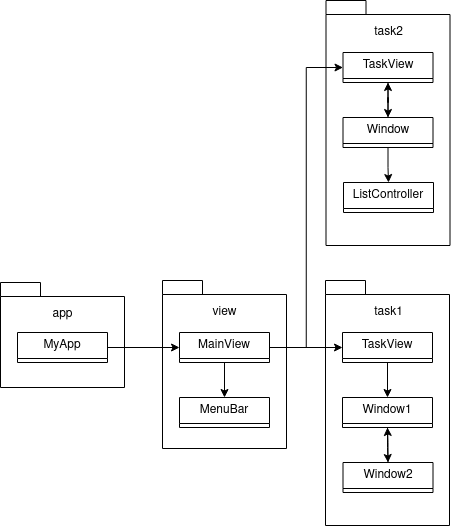
\includegraphics[width=10cm]{1}
\centering
\end{figure}


\section{Висновки:}
Отже, я отримав вміння та навички використовувати інкапсуляцію,
абстракцію типів, успадкування та поліморфізм на основі класів Kotlin
запрограмувавши простий графічний редактор в об’єктно-орієнтованому
стилі.

\end{document}
